\subsection{Understanding bio-physical Coupling}

% (Understand the dynamics bio-physical coupling of oceanographic processes and biological productivity)

In marine environments driven by physical forcing, where abrupt
topographies (e.g. shelf break, canyons) interact with highly dynamic
oceanographic processes, higher nutrient availability due to enhanced
mixing results in higher primary productivity.  The food web in these
regions often supports aggregations of higher predators such as fish,
marine mammals as well as fisheries. In addition to the different
mechanisms that result in increased primary production, there is also
the potential for bio-physical coupled aggregations of zooplankton
that serve as trophic subsidies fueling fish stocks and upper trophic
levels of top predators and marine mammals \cite{genin04}.

Bio-physical coupling between currents and animal behavior are key
factors in the formation of animal aggregations over abrupt
topographies at shallow and intermediate depths. Topographic blockage
(Fig. \ref{fig:plankton}) is suggested as a prevalent mechanism
inducing daily zooplankton accumulations that, in some canyons, are
repeatedly observed at the same site (usually asymmetrically over one
of the canyon edges): 1) during the night the zooplankton migrates
from the deep canyon to the euphotic zone to feed on phytoplankton; 2)
the zooplankton is displaced laterally by the surface circulation; 3)
the topography blocks the morning descent of migrating zooplankton
that accumulates at shallow and intermediate depths.

The bio-geographic, geologic and oceanographic settings of the study
area, accentuated by the presence of the \naz Canyon, induce dynamic
ecological processes and are crucial for supporting high levels of
biological productivity, biodiversity and many ecosystem
services. Much of the local economy is linked to fisheries since
commercially valuable species occur here. Small pelagic fish are among
the most important; these include sardine (\emph{Sardina pilchardus}),
Atlantic mackerel (\emph{Scomber scombrus}), chub mackerel
(\emph{Scomber japonicus}) and horse mackerel (\emph{Trachurus
  trachurus}).

\proj will advance the scientific knowledge of the dynamics of the
oceanographic processes, and the bio-physical coupling that supports
the biological productivity in the study area. Expected observations
will include adaptive sampling by robotic assets especially AUVs, with
continuous acquisition of data on essential ocean variables -- these
include salinity, temperature, oxygen, phytoplankton biomass with
\emph{Chl a} fluorometry as a proxy, and complemented by ship-board
measurements such as nutrients, phytoplankton functional type (using
spectro-fluorescence, flow cytometry and HPLC pigments), photosynthetic
capacity, zooplankton biomass, samples for meta-genomics of phyto and
zooplankton.  The shipboard measurements will be used post-facto to
validate the measurements by the autonomous platforms and model
output.

\begin{wrapfigure}{!h}{3.5in}
  \centering
  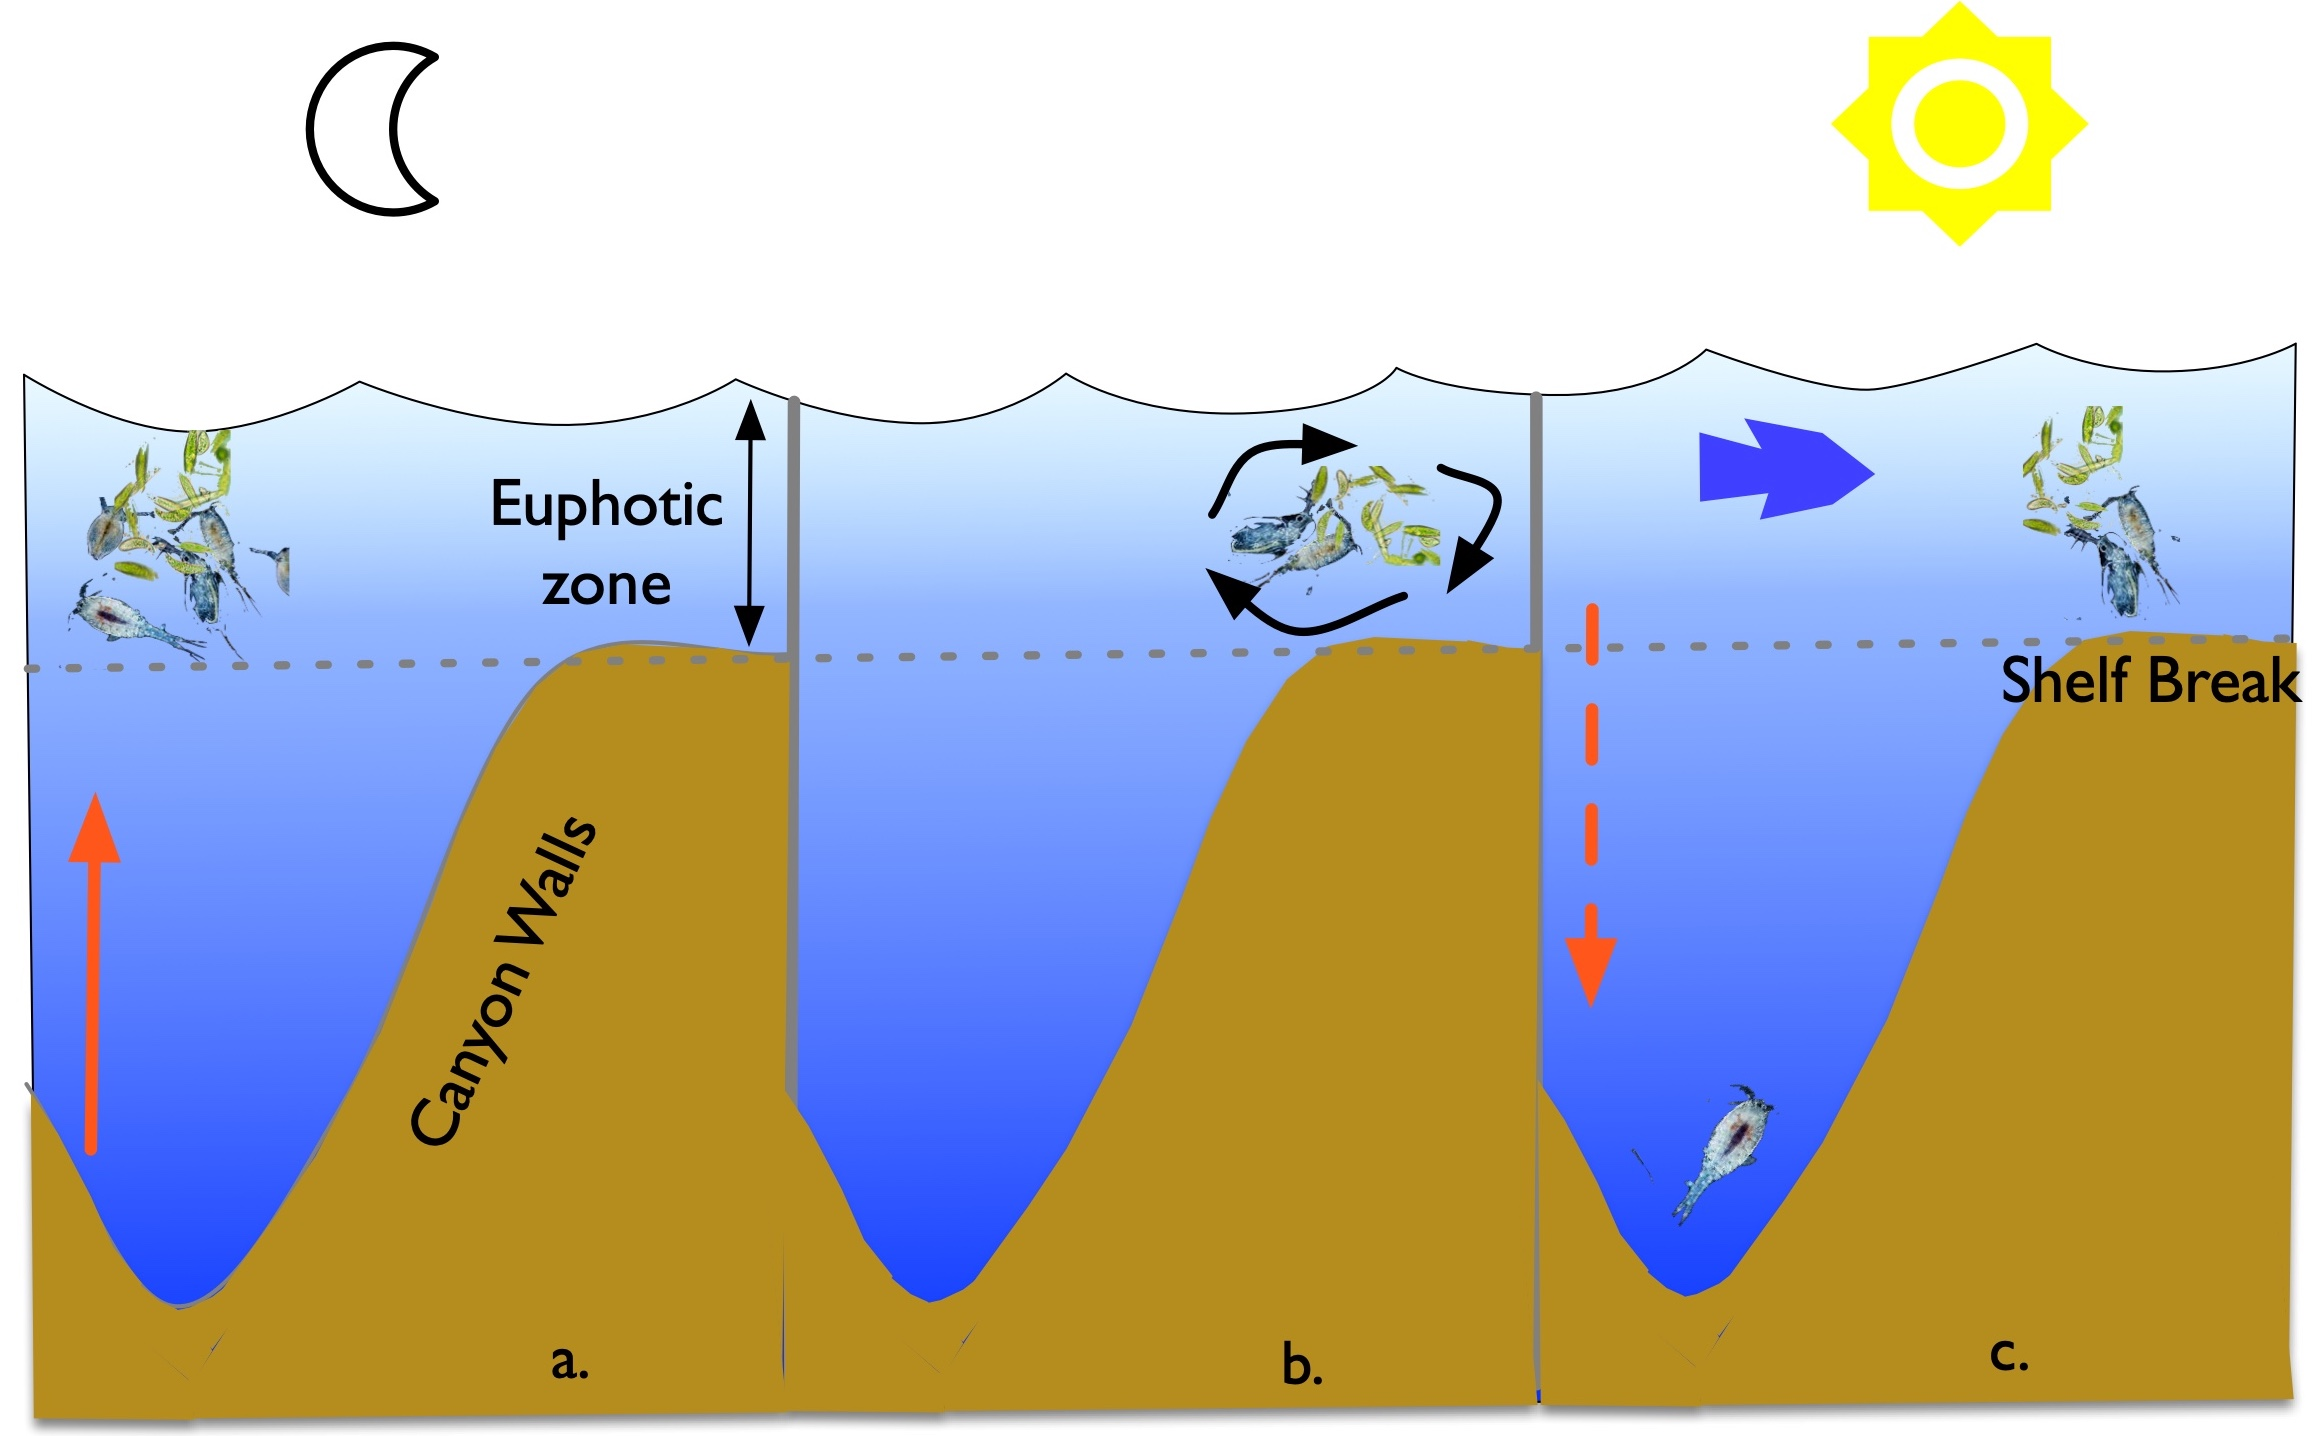
\includegraphics[width=0.5\textwidth]{fig/plankton-canyon.jpg}
  \caption{Bio-physical coupling between currents and animal behavior
    are key factors in the formation of animal aggregations over
    abrupt topographies at shallow and intermediate
    depths. Topographic blockage is suggested as a prevalent mechanism
    inducing daily zooplankton accumulations that, in some canyons,
    are repeatedly observed at the same site (usually asymmetrically
    over one of the canyon edges): 1) during the night the zooplankton
    migrates from the deep canyon to the euphotic zone to feed on
    phytoplankton; 2) the zooplankton is displaced laterally by the
    surface circulation; 3) the topography blocks the morning descent
    of migrating zooplankton that accumulates at shallow and
    intermediate depths.  Red arrows indicate the diel vertical
    migration of zooplankton.}
  \label{fig:plankton}
  \vspace{-1cm}
\end{wrapfigure}

While a fully coupled physical/biological assimilation model is beyond
the scope of this project, \proj will allow the exploration of the
approaches to achieve that end.  Possible extensions of the field
experiment may contribute to the definition of predictive models
helpful for ecosystems management and related bio-economic activities
(e.g. development of a fisheries management advisory tool) based on
our modelling approaches for the \naz Canyon-Berlengas area. These
type of tools are based on (near) real-time ocean data, species
occurrence records and predictive habitat techniques using ecological
niche modelling. The aim would then be to optimize the fishery harvest
of target species while minimizing bycatch and fishery interaction
with non-target species (e.g. marine mammals and turtles).

% \kc{Modelling: primary productivity (maybe can be developed towards
% predicting zooplankton aggregations by integrating ship-board
% measurements?)}

